\documentclass[letterpaper]{article} % DO NOT CHANGE THIS
\usepackage[submission]{aaai2027}  % DO NOT CHANGE THIS
\usepackage[hyphens]{url}  % DO NOT CHANGE THIS
\usepackage{graphicx} % DO NOT CHANGE THIS
\urlstyle{rm} % DO NOT CHANGE THIS
\def\UrlFont{\rm}  % DO NOT CHANGE THIS
\usepackage{natbib}  % DO NOT CHANGE THIS AND DO NOT ADD ANY OPTIONS TO IT
\usepackage{caption} % DO NOT CHANGE THIS AND DO NOT ADD ANY OPTIONS TO IT
\frenchspacing  % DO NOT CHANGE THIS
\usepackage{booktabs}
\pdfinfo{
/TemplateVersion (2027.1)
}
%%MACROS%%
\setcounter{secnumdepth}{1}

\title{Held-Out iAUC Prediction Cannot Validate the Parameters of a Glucose Twin}
\author{
    Anonymous Submission
}
\affiliations{
}

\begin{document}

\maketitle

\begin{abstract}
A personal glucose twin shows a person a fitted parameter, such as insulin sensitivity, and good held-out prediction is the usual reason to trust it. We ask whether that evaluation can warrant the displayed quantity. We fit a Bergman-type simulator to the incremental area under the curve (iAUC) of meals recorded by continuous glucose monitors, and we use a replica in which the model is true so that the answer is known. The area carries almost no information about how a meal's glucose arrives: the weakest Fisher eigenvalue has median \resEigMedianOne{}, and no interval for gastric emptying or carbohydrate absorption is bounded. Insulin sensitivity has a bounded interval for \resSeedsSIBounded\% of replica subjects, and a wrong fixed parameter shifts it with no warning. The fitted model's held-out iAUC error is \resPvpRandomZeroRatio{} times that of the true model on each of two replica seeds whatever its error in the rates, while peak-time and trace error do follow that error. Carbohydrate logging error makes intervals for a combination of the rates more often bounded (\resCvZeroBoundedTau\% to \resCvThreeQuarterBoundedTau\%) and less often right (\resCvZeroCoverTau\% to \resCvThreeQuarterCoverTau\% coverage). We turn these findings into a pre-deployment check.
\end{abstract}

\section{Introduction}

An app that tells a person their insulin sensitivity is low treats a fitted parameter as a measurement. Learned models of glycemic response are judged by how well they predict held-out responses \citep{zeevi2015personalized,berry2020human}, and a mechanistic twin that displays fitted parameters would ordinarily be judged the same way. A model can predict well and still return parameters that mean nothing, so we ask whether predictive evaluation can warrant the quantity that is displayed.

This is an evaluation question that precedes any longitudinal study of what such a display does to a person, because that study assumes the quantity means what its name says. It can be answered without human data. We answer it for one widely used target and one model family, and we measure no human outcome.

The target is the incremental area under the glucose curve (iAUC) of a meal, and the model is a Bergman-type glucose--insulin simulator \citep{bergman1979,dallaman2007} with a two-compartment gut. Three parameters are personal: insulin sensitivity $S_I$, gastric emptying rate $k_e$, and carbohydrate absorption rate $k_a$. We ask which of them the data determine, using the Fisher information matrix, profile-likelihood intervals with fixed definitions of bounded, one-sided and flat \citep{raue2009structural}, and a replica in which the model is exactly true and the subject's own noise and carbohydrate-logging error are reproduced. The replica tells us how often the data would bound a parameter if nothing were wrong with the model.

We make three contributions.
\begin{enumerate}
\item The iAUC carries little information about the timing of glucose entry. This is a classical fact of pharmacokinetics: the mass delivered is fixed, and timing enters an area through the mean absorption time of the gut input \citep{yamaoka1978statistical,cutler1978theory} and, at a finite window, only weakly through its spread. We measure how little, in three cohorts, and show that no profile interval for either gut rate is bounded.
\item Held-out iAUC prediction cannot reveal this. On replicas with random truths, the fit comes within \resPvpRandomZeroRatio{} and \resPvpRandomOneRatio{} times the error of the true model on two seeds while its rates are off by a median root mean squared log error of \resPvpRandomZeroTiming{} and \resPvpRandomOneTiming{}. A check on the peak time or the glucose trace, which the fits were not trained on, does see the error.
\item The replica with input error shows when an interval cannot be believed. Carbohydrate logging error makes intervals for a combination of the two rates more often bounded and less often right, and a wrong fixed parameter is absorbed by $S_I$ with no signal from its interval. We state both as checks that a developer can run.
\end{enumerate}
We do not claim a new fitting method, a clinical result, or that the parameters of any deployed twin are wrong.

\section{Related Work}

Identifiability asks whether unique parameter values can be obtained from data. It is called structural when the question is posed for noise-free output and practical when it is posed for finite, noisy data \citep{cobelli1980parameter,miao2011identifiability,wieland2021structural}. The profile likelihood is a standard practical tool \citep{raue2009structural}, and many fitted models turn out to constrain only combinations of their parameters \citep{gutenkunst2007universally,eisenberg2014determining}. That an area cannot separate two serial rates is a classical result, since flip-flop kinetics hides which of two rates is the slower \citep{boxenbaum1998flipflop}. For glucose models, \citet{erdos2024leveraging} calibrate personal models to continuous glucose monitoring during a glucose tolerance test and report better practical identifiability with the monitored glucose than without it. We differ in two ways. We ask what a prediction check can and cannot see, and we use a replica with input error to learn when a bounded interval can be believed, which a model that is only fitted to real data cannot show.

\section{Setting and Instruments}\label{sec:setting}

\paragraph{Data.} We use three public cohorts of continuous glucose monitoring (CGM) with logged meals: CGMacros \citep{das2025cgmacros} with \resCohortCgmSubjects{} subjects and a median of \resCohortCgmMealsMedian{} meals each, a Shanghai cohort \citep{zhao2023shanghai} with \resCohortShanghaiSubjects{}, and the glucotype study of \citet{hall2018glucotypes} with \resCohortHallSubjects{}. All replica and profile analyses use the \resCohortCgmSubjects{} CGMacros subjects with at least ten logged meals; the other two cohorts enter only the Fisher analysis of Figure~\ref{fig:area}.

\paragraph{Model.} Each meal is simulated alone, starting 30 minutes before it from an empty gut, with the equations
\begin{eqnarray}
\dot Q_1 &=& -k_e Q_1 + m(t),\quad \dot Q_2 = k_e Q_1 - k_a Q_2,\nonumber\\
\dot G &=& -(p_1 + X)\,G + p_1 G_b + k_a Q_2 / V_g,\nonumber\\
\dot I &=& -n\,(I - I_b) + \gamma\,[G - G_b]_+,\nonumber\\
\dot X &=& -p_2 X + p_3 S_I\,(I - I_b),\nonumber
\end{eqnarray}
where $Q_1$ and $Q_2$ are stomach and intestinal glucose, $G$ is plasma glucose, $I$ is plasma insulin, $X$ is remote insulin action, and $m(t)$ is a Gaussian pulse of width two minutes that delivers the glucose mass of the meal. The fixed constants are $p_1=0.026$, $p_2=0.028$, $n=0.16$ and $\gamma=0.16$ per minute, $p_3=1.3\times10^{-5}$, $G_b=90$ mg\,dL$^{-1}$, $I_b=10$ $\mu$U\,mL$^{-1}$, and $V_g=1.6\,W$ dL with body weight $W=78$ kg. The personal parameters have population values $S_I=1$, $k_e=0.026$ and $k_a=0.022$ min$^{-1}$, and each is confined to a box, $[0.3,1.6]$ for $S_I$, $[0.015,0.04]$ for $k_e$ and $[0.012,0.032]$ for $k_a$. The equations are integrated with the Tsit5 solver at relative and absolute tolerance $10^{-4}$ in double precision.

\paragraph{Targets.} The baseline is the mean of the CGM samples in the 30 minutes before the meal, and $y(t)$ is the baseline-subtracted glucose with negative values set to zero. The iAUC is $\int_0^T y\,dt$ over a window $T$ of \resCohortCgmWindow{} minutes (\resCohortHallWindow{} in the Hall study), and the trace is $y$ at the sampling times of the window. The experiments fit different targets, and each section says which. The Fisher and profile analysis of Section~\ref{sec:area}, the prediction comparison of Section~\ref{sec:prediction} and the perturbation of Section~\ref{sec:absorb} fit the iAUC. The combination of the rates (Section~\ref{sec:input}) and the symmetry control (Section~\ref{sec:symmetry}) fit the full trace.

\paragraph{Likelihood and estimation.} Residuals are Gaussian with a standard deviation per subject and target and, for the trace, a first-order autocorrelation, and the trace residuals are whitened for it (Prais--Winsten). Both are estimated at a pilot fit and then frozen, because re-estimating them inside the optimization would let a fit lower its loss by calling its errors noise. In a replica the pilot fit uses the replica data, so the estimated standard deviation includes whatever the input error adds to the residual. Parameters are estimated by maximum likelihood in logarithmic coordinates, with a gradient fit followed by an L-BFGS-B polish. Thirty random starts in place of five leave the polished likelihood within the interval cutoff of the earlier one for \resGlobalWithinCount{} of \resGlobalN{} real subjects, so we treat the polished estimate as the optimum. The fits used for prediction minimize the squared iAUC error with a small penalty toward the population values, and every identifiability analysis uses the unpenalized likelihood.

\paragraph{Held-out prediction.} We use five repeats of five-fold cross-validation within subject. Meals are assigned to folds at random with a seeded hash, identically for all methods, so a held-out meal can fall between training meals in time.

\paragraph{Intervals.} A profile interval is the set of values whose profile negative log-likelihood is within $\resDeltaThreshold{}$ of its minimum. It is bounded if the profile exceeds that level on both sides inside the parameter box, one-sided if on one side, and flat if on neither. Only bounded counts as identified. We call this rule the profile classifier. A subject is interior for a parameter if its estimate is more than one percent of the box from both bounds. We report the bounded fraction over interior subjects, because an estimate on a bound has no interval to classify, and over all subjects where it matters.

\paragraph{Replica and floor.} In the replica, each subject's fitted parameters are the truth. Every real meal is simulated at the truth, autocorrelated noise with the subject's own variance is added, and the fit receives the logged carbohydrate times a lognormal error with coefficient of variation 0.25. A replica set is one seed unless stated, and fractions carry Wilson intervals. The floor is the held-out error of the model at the true parameters, so a ratio to the floor measures what is lost to the parameters alone. Spearman correlations $\rho_s$ carry bootstrap intervals over subjects.

\section{What an Area Can See}\label{sec:area}

For a unit meal and an empty gut, the density of gut appearance has first moment $\tau_1 = 1/k_e + 1/k_a$ and second moment set by $q = 1/(k_e k_a)$. An area over a long window sees the total mass, which is the same for every pair of rates. At a finite window it sees timing only through the share of the mass delivered by the window's end and through what leaks past it, so the area depends on $\tau_1$ and, weakly, on $q$. Exchanging $k_e$ and $k_a$ leaves $\tau_1$ and $q$ unchanged. The cascade is linear, so the symmetry is exact, and the simulated glucose differs by at most \resGutSweepMaxZero{} mg\,dL$^{-1}$, which is solver tolerance.

Figure~\ref{fig:area}a shows the iAUC over the physiological box of the two rates for a \figMealGrams{} g meal and a \figWindowMin{} minute window. The whole box spans \figIaucSurfaceRange{} mg\,min\,dL$^{-1}$, which is \figIaucRangeOverNoise{} of the standard deviation of the iAUC noise of a single meal in CGMacros (median \figIaucNoiseSd{}). Three rate pairs with the same $\tau_1$ of \figPairTauOne{} minutes and $q$ from \figPairPA{} to \figPairPC{} differ in iAUC by \figPairIaucSpreadPct\%, in peak time by \figPairPeakTimeSpread{} minutes and in peak glucose by \figPairPeakGlucoseSpread{} mg\,dL$^{-1}$ (Figure~\ref{fig:area}b). Their traces differ by at most \figPairTraceMaxDiff{} mg\,dL$^{-1}$, against a noise standard deviation of \figTraceNoiseSd{} per CGM reading.

\begin{figure*}[t]
\centering
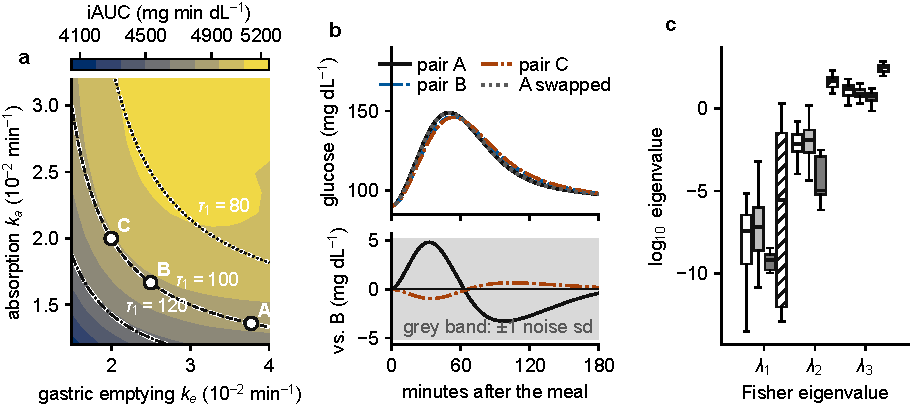
\includegraphics[width=0.95\textwidth]{figures/fig_area}
\caption{What an area can see. \textbf{(a)} iAUC over the physiological box of $k_e$ and $k_a$; dashed lines are rate pairs of equal $\tau_1$, and the circles are the pairs A, B and C plotted in (b). \textbf{(b)} Glucose for three pairs with $\tau_1=\figPairTauOne{}$ min, pair A also with its rates swapped, and the difference from pair B, with one noise standard deviation of a CGM reading in grey. \textbf{(c)} Fisher eigenvalues at the primary box, weakest first, under the iAUC for CGMacros (white), Shanghai (light grey) and Hall (dark grey), and under the full trace for CGMacros (hatched).}
\label{fig:area}
\end{figure*}

We see the same thing in the Fisher information, subject by subject. Its median eigenvalues under the iAUC are \resEigMedianOne{}, \resEigMedianTwo{} and \resEigMedianThree{}, and under the full trace they are \figEigTraceMedianOne{}, \figEigTraceMedianTwo{} and \figEigTraceMedianThree{} (Figure~\ref{fig:area}c), so the trace constrains every direction more tightly. The iAUC profile intervals agree with the spectrum. At the primary box the interval for $k_e$ is bounded in \figRealIaucKeBoundedAll{} of \figRealIaucN{} subjects and the interval for $k_a$ in \figRealIaucKaBoundedAll{}. Insulin sensitivity is bounded for \figRealIaucSIBoundedAll{} of \figRealIaucN{} subjects, which is \resProfileIaucSIInteriorBoundedOne{} of the \resProfileIaucSIInteriorNOne{} interior subjects (\resProfileIaucSIInteriorFracOne\%, Wilson interval \resProfileIaucSIInteriorFracOneLow{} to \resProfileIaucSIInteriorFracOneHigh\%). When the model is exactly true the fraction among interior subjects is \resSeedsSIBounded\% over five replica seeds (\resSeedsSIBoundedCount{} of \resSeedsSIInterior{} subject-seed pairs). On one seed it is \resNoiseOneIaucSI\% at the estimated noise and \resNoiseQuarterIaucSI\% when the noise is cut to a quarter, so the weakness of $S_I$ is partly a property of the noise level and partly of the target.

\section{Prediction Does Not See It}\label{sec:prediction}

The fits in this section are to the iAUC, and we evaluate them on the iAUC and on two targets they were not trained on, the peak time and the trace. On the real data, the twin predicts the held-out iAUC better than a model-free personal mean, with a mean absolute error of \resMaeGradThree{} against \resMaePersonalMean{} mg\,min\,dL$^{-1}$. Fitting the full trace instead of the iAUC gives \resMaeGradThreeTrace{}. The advantage over the personal mean does not depend on random folds. The error of the three-parameter fit differs from that of the personal mean by $\resDiffGradThreeVsPersonalMean{}$ with random folds, by $\figChronoBlockedPersonalMean{}$ ($\figChronoBlockedPersonalMeanLow{}$ to $\figChronoBlockedPersonalMeanHigh{}$) with blocked chronological folds, and by $\figChronoForwardPersonalMean{}$ ($\figChronoForwardPersonalMeanLow{}$ to $\figChronoForwardPersonalMeanHigh{}$) when only earlier meals train. Gradient fitting and a grid search over the parameters differ by $\resDiffGradThreeVsGridThree{}$ mg\,min\,dL$^{-1}$ (95\% interval $\resDiffGradThreeVsGridThreeLow{}$ to $\resDiffGradThreeVsGridThreeHigh{}$), and fitting all three parameters instead of $S_I$ alone changes the error by $\resDiffGradThreeVsGradOne{}$ ($\resDiffGradThreeVsGradOneLow{}$ to $\resDiffGradThreeVsGradOneHigh{}$), a small gain. Real data cannot say what these small differences hide, because the true parameters are unknown.

The replica can. We drew true parameters at random across the box and fitted the replica data. On each of two seeds the fitted model's held-out iAUC error is \resPvpRandomZeroRatio{} and \resPvpRandomOneRatio{} times the floor, while the rates are off by a median root mean squared log error of \resPvpRandomZeroTiming{} and \resPvpRandomOneTiming{} (Figure~\ref{fig:prediction}a). Across subjects the ratio is unrelated to the rate error: the Spearman correlation is $\resPvpRandomZeroRhoTimingRatio{}$ ($\resPvpRandomZeroRhoTimingRatioLow{}$ to $\resPvpRandomZeroRhoTimingRatioHigh{}$) on seed zero and \figPvpRhoIauc{} pooled over both seeds. With \resPvpRandomZeroN{} subjects per seed, a moderate correlation cannot be excluded, but the median ratio stays near one across the whole range of rate error we drew.

Targets the fits were not trained on do register the error. On seed zero the free-timing fit is \resFloorPeakRandomZeroThreeRatio{} times the floor for the peak time and \resFloorTraceRandomZeroThreeRatio{} times for the glucose trace, and its excess rises with the rate error (Spearman \resFloorPeakRandomZeroThreeRho{} and \resFloorTraceRandomZeroThreeRho{}, and \figPvpRhoPeak{} and \figPvpRhoTrace{} pooled over both seeds, as plotted in Figure~\ref{fig:prediction}). The fit of $S_I$ alone, with population rates, sits at \resFloorPeakRandomZeroOneRatio{} and \resFloorTraceRandomZeroOneRatio{} times the floor and shows no such trend. This is the cost of fitting rates that the iAUC does not determine: it is invisible on the training target and visible elsewhere. A prediction check on the training target cannot separate a twin with good parameters from one with bad ones, and a check on peak time or trace can.

\begin{figure*}[t]
\centering
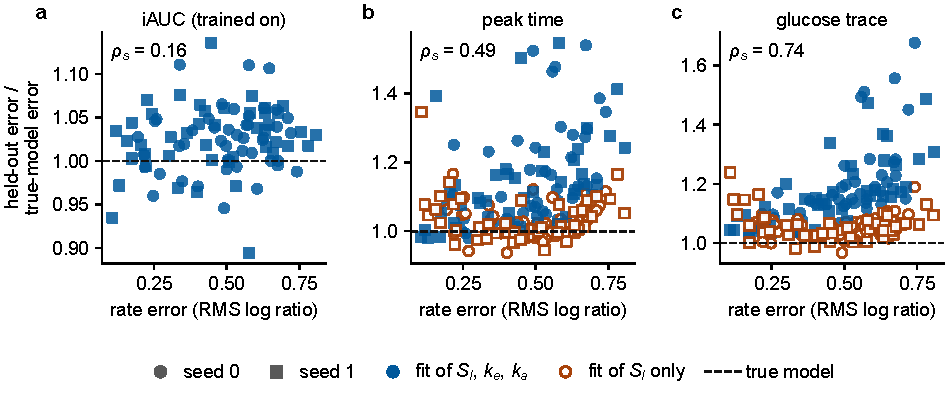
\includegraphics[width=0.95\textwidth]{figures/fig_prediction}
\caption{Held-out error against the error of the rates on true-model replicas with random truths, two seeds pooled; the fits are to the iAUC. Each point is a subject, and the dashed line is the error of the true model. \textbf{(a)} iAUC, the target the fits were trained on. \textbf{(b)} Peak time. \textbf{(c)} Glucose trace. Filled marks are fits of $S_I$, $k_e$ and $k_a$; hollow marks are fits of $S_I$ alone with population rates. $\rho_s$ is the Spearman correlation of the fit of all three parameters.}
\label{fig:prediction}
\end{figure*}

\section{Input Error Makes Intervals Bounded and Wrong}\label{sec:input}

The exchange symmetry leaves a combination of the rates free, $\tau_1$ and $q$, and the full glucose trace carries more information about it than the area does. The experiments in this section fit the full trace, whitened, in logarithmic coordinates with polished estimates, and ask when the interval for the combination can be believed. We sweep the coefficient of variation of the carbohydrate logging error on the replica (Figure~\ref{fig:sweep}). With exact carbohydrate, the intervals for $\tau_1$ and $q$ are bounded for \resCvZeroBoundedTau\% and \resCvZeroBoundedP\% of interior subjects (\figSweepAllTauBoundedExact{} and \figSweepAllQBoundedExact{} of \figSweepAllNExact{} subjects overall) and cover the truth for \resCvZeroCoverTau\% and \resCvZeroCoverP\%. At a coefficient of variation of $0.25$ they are bounded for \resCvQuarterBoundedTau\% and \resCvQuarterBoundedP\% (\figSweepAllTauBoundedQuarter{} and \figSweepAllQBoundedQuarter{} of \figSweepAllNQuarter{} overall) and cover for \resCvQuarterCoverTau\% and \resCvQuarterCoverP\%. At $0.75$ the bounded fractions reach \resCvThreeQuarterBoundedTau\% and \resCvThreeQuarterBoundedP\% (\figSweepAllTauBoundedThreeQuarter{} and \figSweepAllQBoundedThreeQuarter{} of \figSweepAllNThreeQuarter{} overall) while coverage falls to \resCvThreeQuarterCoverTau\% and \resCvThreeQuarterCoverP\%. All fractions rise or fall in the same direction over interior and over all subjects.

\begin{figure}[t]
\centering
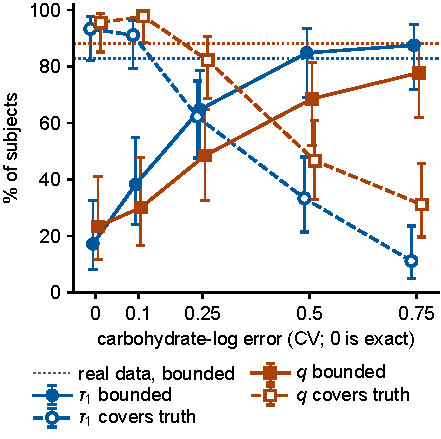
\includegraphics[width=0.97\columnwidth]{figures/fig_sweep}
\caption{The combination $(\tau_1,q)$ on one replica seed as the carbohydrate logging error grows; the fits are to the full trace. Solid lines: share of interior subjects with a bounded interval, with Wilson intervals. Dashed lines: share of all subjects whose nominal interval contains the truth, with Wilson intervals. Dotted lines: bounded shares on the real data.}
\label{fig:sweep}
\end{figure}

Why does input error make intervals narrower and wrong? The fitted parameters absorb a mismatch in the carbohydrate input, so the residual does not grow: the median pilot noise estimate changes by \figSweepSigmaChangePct\% between exact carbohydrate and an error of 0.1. The likelihood is as curved as before, and its interval does not widen, while the estimate moves by more than the interval. We make this concrete by asking what interval would cover the truth. For a cutoff that covers the truth for 90\% of subjects, the noise standard deviation would have to be \figSweepSigmaTauQuarter{} times larger at an error of $0.25$ and \figSweepSigmaTauThreeQuarter{} times larger at $0.75$ for $\tau_1$, and at those cutoffs the intervals are bounded for only \figSweepCalBoundedTauQuarter\% and \figSweepCalBoundedTauThreeQuarter\% of interior subjects. The bounded intervals at the nominal level reflect the likelihood treating the logged carbohydrate as exact. Two further checks agree. Estimating the noise standard deviation and autocorrelation again at the polished estimate changes nothing: the nominal interval covers the truth for \figFinalCoverTauQuarter\% and \figFinalCoverQQuarter\% of subjects at an error of $0.25$ and for \figFinalCoverTauThreeQuarter\% and \figFinalCoverQThreeQuarter\% at $0.75$, the same as with the pilot estimate. And a systematic error, one multiplier per subject shared by every meal, with a coefficient of variation of $0.25$, breaks the intervals as well: they are bounded for \figSysBoundedTau\% and \figSysBoundedQ\% and cover for \figSysCoverTau\% and \figSysCoverQ\%, so an error that only rescales the carbohydrate is not absorbed by $S_I$ either. The pattern replicates on two further replica seeds. For $\tau_1$ the bounded share rises from \figSeedOneTauBoundedZero\% and \figSeedTwoTauBoundedZero\% at exact carbohydrate to \figSeedOneTauBoundedHigh\% and \figSeedTwoTauBoundedHigh\% at $0.75$ while coverage falls from \figSeedOneTauCoverZero\% and \figSeedTwoTauCoverZero\% to \figSeedOneTauCoverHigh\% and \figSeedTwoTauCoverHigh\%, and for $q$ the rise is at least \figSeedMinRiseQ{} points and the fall at least \figSeedMinDropQ{} points. We have no mechanism for why the bounded share rises with the error, as well as for why the coverage falls. A sandwich or bootstrap interval is the natural repair, and we did not test one.

On the real data the intervals are bounded for \resPolishedBoundedTauTrace\% and \resPolishedBoundedPTrace\% of interior subjects, which is what a replica with a large input error produces. We cannot say that input error is the cause, because misfit or sensor lag would produce the same pattern, but it shows that a bounded interval on real data is not evidence that the quantity is known.

The classifier can identify the combination when the data and the inputs allow it. With exact carbohydrate and a quarter of the replica noise, and a profile computed to convergence on a finer grid, the intervals are bounded for \resConvFineTauBounded\% and \resConvFinePBounded\% of subjects and cover the truth for \resConvFineTauCover\% and \resConvFinePCover\%. This check also corrected one of our own results. Read off a coarse grid, the same profiles seemed to miss the truth: the excess at the true value of $\tau_1$ was above the cutoff for \resTruthQuarterTauStoredOver\% of subjects. Computed directly at the true value, it was above the cutoff for \resTruthQuarterTauDirectOver\% for $\tau_1$. The grid had interpolated a narrow profile, and the likelihood was calibrated all along. A classifier should be tested against the likelihood at the truth before its intervals are trusted.

\section{A Wrong Fixed Parameter Is Absorbed}\label{sec:absorb}

In the model equations, insulin above its basal level is proportional to the secretion gain $\gamma$, and it drives the action state through $p_3 S_I$. The glucose trace therefore depends on $\gamma$, $p_3$ and $S_I$ only through the product $\gamma\,p_3\,S_I$, and scaling either fixed parameter is the same as scaling $S_I$. That identity predicts the shift of the estimate. What it does not predict is what the interval and the box do, which is what this section measures, with fits to the iAUC. We multiplied $\gamma$ in the truth of the standard replica by $1.3$ and by $0.7$ and kept the population value in the fit.

The estimate of $S_I$ absorbs the change in the direction the scale predicts, and only while it stays inside its box (Figure~\ref{fig:absorb}): at $0.7$, \figAbsorbPinnedZeroSeven{} estimates end on a bound against \figAbsorbPinnedOne{} on the unperturbed replica. The unperturbed median is not zero, and the reason is not carbohydrate error. With exact carbohydrate the median of the log ratio is \figAbsorbMedianExact{} with \figAbsorbPinnedExact{} of \figAbsorbNExact{} estimates on a bound, because the replica truths lie near the edges of the box.

The interval does not signal the error. On the unperturbed replica the nominal interval for $S_I$ contains the truth for \resPertBaseSICover\% of subjects and, at $0.7$, for \resPertGammaDownSICover\%, while the share of bounded intervals goes from \resPertBaseSIBounded\% to \resPertGammaDownSIBounded\%. We read $S_I$ as a scale of insulin action, not as a property of the person, and a developer who shows it as the second should say what was held fixed.

\begin{figure}[t]
\centering
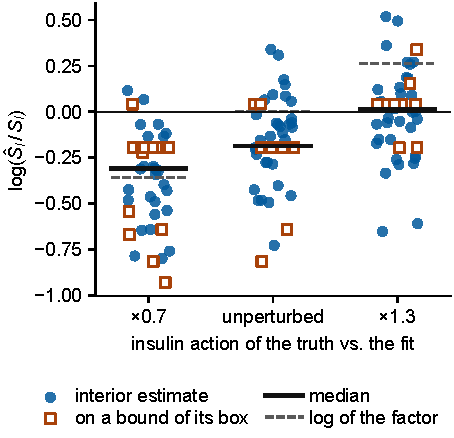
\includegraphics[width=0.97\columnwidth]{figures/fig_absorption}
\caption{Log ratio of the estimate of $S_I$ to its truth when the truth's insulin secretion is multiplied by $0.7$, left unchanged or multiplied by $1.3$, with the fit keeping the population value; fits to the iAUC on the standard replica. Squares are estimates on a bound of their box, the black bar is the median over \figAbsorbNOne{} subjects, and the dashed line is the logarithm of the factor.}
\label{fig:absorb}
\end{figure}

\section{Breaking the Symmetry Is Not Enough}\label{sec:symmetry}

If the exchange symmetry were the only reason the gut rates are not bounded, a design that breaks it should bound them. We gave every meal of a random-truth replica a known residual intestinal content, equal in the truth and the fit so that the model stays exactly true, and fitted the full trace in rate coordinates. At a content of $10\%$ of the meal, $k_e$ and $k_a$ are bounded for \resResTenKeBounded\% and \resResTenKaBounded\% of interior subjects, with coverage of \resResTenKeCover\% and \resResTenKaCover\%. At $20\%$ the shares are \resResTwentyKeBounded\% and \resResTwentyKaBounded\%. The rule we set before the run asked for at least half bounded and ninety percent covered at ten percent, and it was not met. Breaking the symmetry helps in proportion to the residue, but a structural result that the rates are separable does not give a bounded interval at this noise.

\begin{table*}[t]
\centering
\small
\begin{tabular}{lllr}
\toprule
check & target & result & subjects \\
\midrule
Fisher eigenvalues, medians & iAUC & \resEigMedianOne{}, \resEigMedianTwo{}, \resEigMedianThree{} & \resCohortCgmSubjects{} \\
Fisher eigenvalues, medians & trace & \figEigTraceMedianOne{}, \figEigTraceMedianTwo{}, \figEigTraceMedianThree{} & \resCohortCgmSubjects{} \\
Bounded interval for $k_e$ and $k_a$ & iAUC & \figRealIaucKeBoundedAll{} and \figRealIaucKaBoundedAll{} (upper limits \resProfileIaucKeOneHigh\% and \resProfileIaucKaOneHigh\%) & \figRealIaucN{} \\
Bounded interval for $S_I$, real & iAUC & \resProfileIaucSIInteriorFracOne\% of interior; \figRealIaucSIBoundedAll{} of \figRealIaucN{} overall & \resProfileIaucSIInteriorNOne{} interior \\
Bounded interval for $S_I$, replica & iAUC & \resSeedsSIBounded\% of interior, five seeds & \resSeedsSIInterior{} interior pairs \\
Held-out error over the floor & iAUC (trained) & \resPvpRandomZeroRatio{} and \resPvpRandomOneRatio{} on two seeds; rate error \resPvpRandomZeroTiming{} and \resPvpRandomOneTiming{} & \resPvpRandomZeroN{} per seed \\
Peak-time and trace error over the floor & iAUC fits & free-timing fit \resFloorPeakRandomZeroThreeRatio{} and \resFloorTraceRandomZeroThreeRatio{}; $S_I$-only \resFloorPeakRandomZeroOneRatio{} and \resFloorTraceRandomZeroOneRatio{} & \resPvpRandomZeroN{} \\
$(\tau_1,q)$ bounded, exact carbohydrate & trace & \resCvZeroBoundedTau\% and \resCvZeroBoundedP\% of interior, covering \resCvZeroCoverTau\% and \resCvZeroCoverP\% & \resCohortCgmSubjects{} \\
$(\tau_1,q)$ bounded, error 0.75 & trace & \resCvThreeQuarterBoundedTau\% and \resCvThreeQuarterBoundedP\%, covering \resCvThreeQuarterCoverTau\% and \resCvThreeQuarterCoverP\% & \resCohortCgmSubjects{} \\
$S_I$ covers the truth, $\gamma$ scaled by $0.7$ & iAUC & \resPertBaseSICover\% unperturbed, \resPertGammaDownSICover\% perturbed & \resCohortCgmSubjects{} \\
$k_e$ and $k_a$ bounded, residual gut $10\%$ & trace & \resResTenKeBounded\% and \resResTenKaBounded\% of interior & \resCohortCgmSubjects{} \\
\bottomrule
\end{tabular}
\caption{Headline numbers, with the target each check fits. Bounded fractions are over interior subjects unless the row says overall; the floor is the held-out error of the model at the true parameters; replica rows are one seed unless stated.}
\label{tab:main}
\end{table*}

\section{A Pre-Deployment Check}

The analyses above are the steps of a check that can precede a study of what a parameter display does to a person.
\begin{enumerate}
\item Compute the Fisher information and profile intervals for every parameter that will be shown, and report bounded, one-sided and flat intervals separately, with the box that defines them, over interior and over all subjects.
\item Run a replica in which the model is true and in which the inputs carry an error of the size to be expected, then report how often the intervals are bounded and how often they contain the truth, with the error varied.
\item Measure the error of the fit against the error of the true model on targets the fit was not trained on, such as peak time and trace, because the training target cannot show it.
\item Perturb each fixed parameter and report what the displayed parameter absorbs, and compare the classifier with the likelihood at the truth.
\end{enumerate}
Each step needs only the simulator and the subjects' own data.

\section{Implications for Evaluating AI Interventions}

A prediction metric is a surrogate for the thing a system shows a person, and here the two come apart: the surrogate is flat in the quantity that is displayed. The same structure appears wherever a personalized system reports a latent state, such as a skill estimate, a risk factor or a physiological parameter, and evaluates itself by how well it predicts the next observation. A study of the effects of such a display on behavior over time then rests on a quantity whose meaning was never checked. We suggest that evaluations of such systems record which quantity was shown, what was held fixed in its estimate, and whether a replica with realistic input error would have bounded it.

\section{Limitations}

\paragraph{One model family, one estimator class.} We study a single Bergman-type simulator, the iAUC and the full trace, and three small cohorts, and the replica reuses CGMacros meal schedules. Only CGMacros enters the replica and profile analyses; Shanghai and Hall enter only the Fisher analysis. We tested a classical maximum-likelihood estimator and no learned or amortized estimator, so we cannot say whether those fail in the same way.

\paragraph{Seeds.} The sweep over input error replicates on three replica seeds. The perturbation of $\gamma$, the residual-content control and the check against the likelihood at the truth each use one seed, and only the fraction for $S_I$ is pooled over five seeds.

\paragraph{Input error.} The replica draws an independent lognormal error with coefficient of variation 0.25. Real logging error is probably systematic, and the sweep shows that the answer depends on its size. We did not test a systematic error model or a sandwich interval.

\paragraph{Fixed physiology.} Basal glucose is a constant in the simulator, and the model has no sensor lag. A timing parameter can absorb either, which would affect the real-data fractions but not the replica, where the model is true by construction.

\paragraph{Splits.} Most cross-validation folds are random within subject, so autocorrelation between neighboring meals is not removed. The chronological folds of Section~\ref{sec:prediction} are on one cohort.

\paragraph{Scope of the human claim.} We measure the validity of a displayed quantity and no human outcome. We do not show that a person who sees an unreliable parameter is harmed, or that a reliable one helps.

\section*{Ethical Statement}

All data are public and de-identified, and we collected none. The model is a research simulator that has not been validated for clinical use, and nothing here should inform a medical decision.

[AUTHOR: AI-use statement to be completed by the authors, giving the tool, the tasks it performed, and what the authors verified.]

\bibliography{caleai}

\end{document}
